\documentclass{article}
% Language setting
% Replace `english' with e.g. `spanish' to change the document language
\usepackage[english]{babel}
\usepackage{booktabs}
\usepackage{float} % for H specifier

% Set page size and margins
% Replace `letterpaper' with `a4paper' for UK/EU standard size
\usepackage[letterpaper,top=2cm,bottom=2cm,left=3cm,right=3cm,marginparwidth=1.75cm]{geometry}

% Useful packages
\usepackage{amsmath}
\usepackage{graphicx}
\usepackage[colorlinks=true, allcolors=blue]{hyperref}

\begin{document}

\title{NIFTY 50 Stock Price Prediction \& Pairs Trading Classification}
\author{Aditya Moza 2022035 \and Manit Kaushik 2022277}
\date{} % Remove the date

\maketitle

\section{Introduction}

The objective of our project is to do an analysis of the stock prices of companies listed in the NIFTY 50 index using machine learning techniques. The NIFTY 50 index comprises India's top 50 companies across various sectors, making it a significant benchmark for the Indian stock market. This project is divided into three main sections: stock price prediction, stock classification based on growth, and classification of profitable pairs for pairs trading. The datasets used for our project is \href{https://www.kaggle.com/datasets/rohanrao/nifty50-stock-market-data/data}{NIFTY-50 Stock Market Data (2000 - 2021)} and the Yahoo Finance Python API. 

\section{Background}
Analyzing stock prices in the NIFTY 50 index holds significant relevance for investors, analysts, and policymakers alike. Understanding the dynamics of these leading companies provides insights into broader market trends, economic conditions, and investment opportunities within India's stock market landscape.

Numerous studies have explored stock price prediction and classification using machine learning methods, particularly in the context of financial markets. Research often encompasses various algorithms, including regression models, neural networks, and ensemble methods, to forecast stock prices and classify stocks based on growth potential. Additionally, the concept of pairs trading, aimed at exploiting market inefficiencies, has been extensively studied, with researchers investigating diverse strategies and methodologies to identify profitable pairs.


\section{Stock Price Prediction}

For this task, we have implemented and compared between three well-known Machine Learning techniques, Convolutional Neural Network Long Short-Term Memory Model (\textbf{CNN-LSTM}), K-Nearest Neighbours (\textbf{KNN}) \& Multi-Linear Regression (\textbf{MLR}). We have presented our findings for this section using TCS Stock.

\begin{figure}[H]
    \centering
    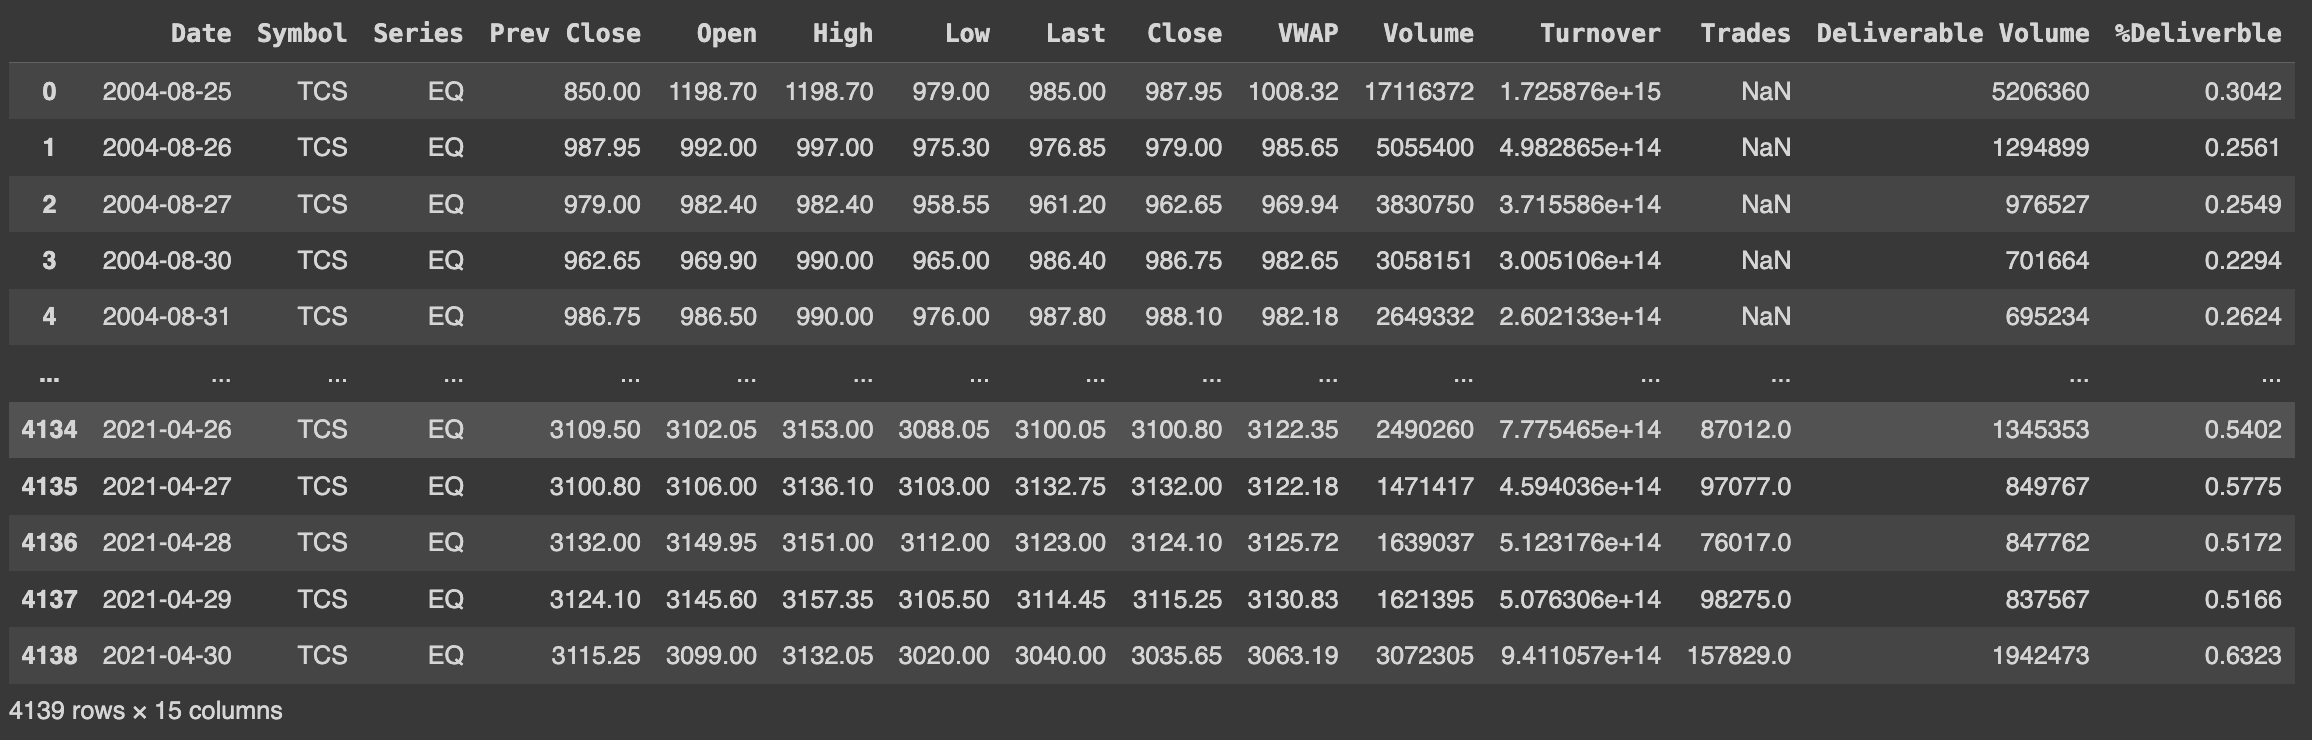
\includegraphics[width=1.0\linewidth]{data_table_tcs.png}
    \label{fig:enter-label}
\end{figure}

\subsection{CNN-LSTM}

This model employs a short history of a stock, utilizing the prices of the previous 5 days as features to forecast future prices. It adopts a hybrid architecture, integrating Convolutional Neural Networks (CNNs) with an LSTM layer, followed by a linear layer for prediction. The model is trained using mean squared error loss and the Adam optimizer over 20 epochs.

\begin{table}[htbp]
    \centering
    \caption{LSTM Data Table Used}
    \label{tab:close_history}
    \begin{tabular}{ccccccc}
        \toprule
        Date & Close & Close t-1 & Close t-2 & Close t-3 & Close t-4 & Close t-5 \\
        \midrule
        2004-09-01 & 987.90 & 988.10 & 986.75 & 962.65 & 979.00 & 987.95 \\
        2004-09-02 & 993.65 & 987.90 & 988.10 & 986.75 & 962.65 & 979.00 \\
        2004-09-03 & 997.85 & 993.65 & 987.90 & 988.10 & 986.75 & 962.65 \\
        \bottomrule
    \end{tabular}
\end{table}

% \begin{table}[h]
%     \centering
%     \begin{tabular}{l c} % Adjust column alignment as needed
%         \toprule
%         \textbf{Dataset} & \textbf{MSE [0,1]} \\
%         \midrule
%         \emph{Train} & \textbf{0.02150464} \\
%         \emph{Test} & \textbf{0.04678102} \\
%         \bottomrule
%     \end{tabular}
%     \label{tab:mean_squared_error}
% \end{table}

\begin{figure}[H]
    \centering
    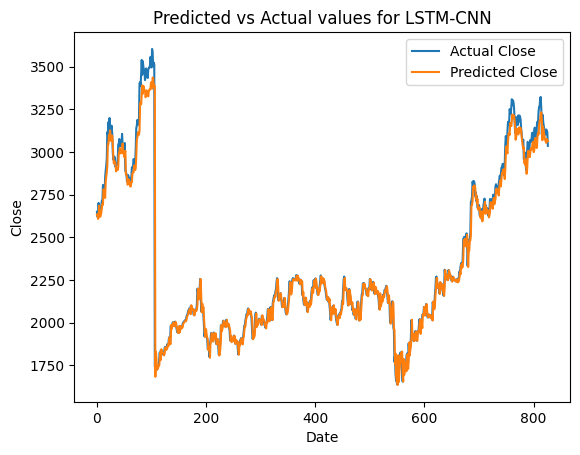
\includegraphics[width=0.6\linewidth]{cnn_test.png}
    \label{fig:enter-label}
\end{figure}

\subsection{Multi-Linear Regression}

In this method, a multi-linear regression (MLR) model is applied to predict the Close Price of a stock using various features including "Open," "High," "Low," "Volume," and "Turnover" from the dataset.

\begin{figure}[H]
    \centering
    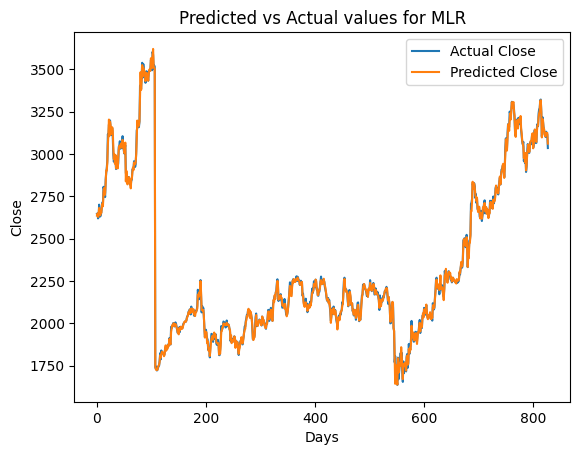
\includegraphics[width=0.6\linewidth]{mlr_test.png}
    \label{fig:enter-label}
\end{figure}

\subsection{K-Nearest Neighbours}
In this method, the K-Nearest Neighbors Regression (KNN) algorithm is applied for predicting the stock's closing price. The KNN algorithm works by finding the 'k' nearest data points in the feature space and averaging their target values to make predictions.

\begin{figure}[H]
    \centering
    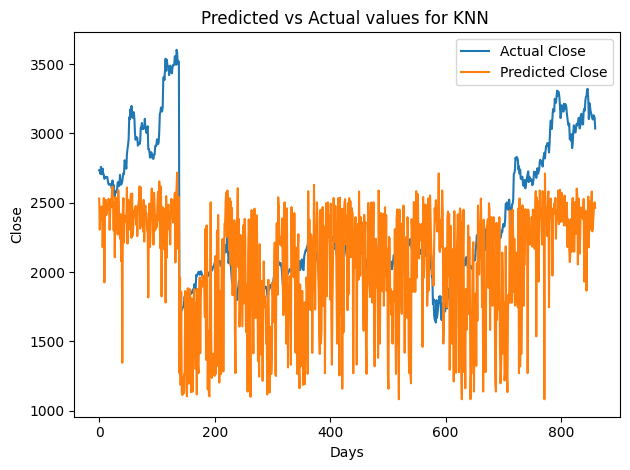
\includegraphics[width=0.6\linewidth]{knn_test_reg.png}
    \label{fig:enter-label}
\end{figure}

\begin{table}[h]
    \centering
    \begin{tabular}{l c} 
        \toprule
        \textbf{Method} & \textbf{MSE on Test Dataset} \\
        \midrule
        \emph{CNN-LSTM} & \textbf{0.04678102} \\
        \emph{MLR} & \textbf{0.00010230} \\
        \emph{KNN} & \textbf{0.41147872} \\
        \bottomrule
    \end{tabular}
    \label{tab:mean_squared_error}
\end{table}

From the Predicted v/s Actual Values Graphs and the MSE Errors Table, we can conclude that for this dataset our MLR Model performs the best out of the three models created and KNN performs the worst.

\section{Stock Classification Based on Growth}
In this section, we have used K Nearest Neighbours and Decision Trees to classify whether the price of a stock will go higher than the price of previous of day or lower. 

\subsection{K-Nearest Neighbours}
In this method, the K-Nearest Neighbors (KNN) algorithm is used for a classification problem. The objective is to predict whether to Buy (+1) or Sell (-1), essentially predicting whether the stock will rise or fall. The results are as follows:

\begin{figure}[H]
    \centering
    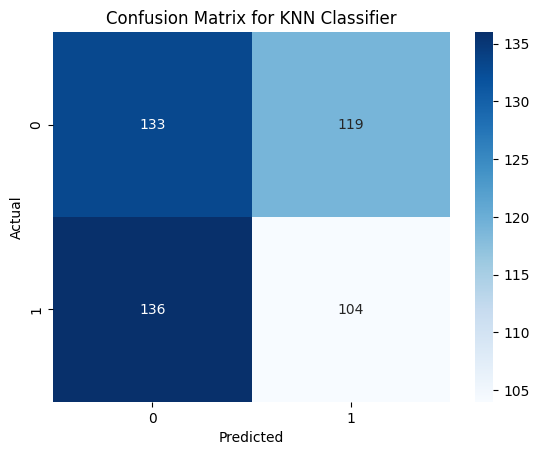
\includegraphics[width=0.45\linewidth]{cnfmat_knn.png}
    \label{fig:enter-label}
\end{figure}

\subsection{Decision Trees}
In this method, a Decision Trees Classifier is employed to predict stock price movements based on features such as "Open - Close," "High - Low," "Volume," and "Turnover." The target variable is determined by comparing the closing price of the current day with that of the next day. The labels of +1 and -1 mean the same here as it did in the KNN Model. Since this model gives a different result every time we took the average of training and testing accuracies over 100 epochs. The results are as follows:

\begin{figure}[H]
    \centering
    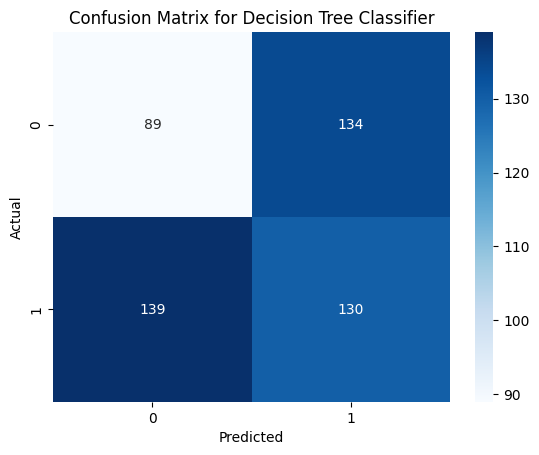
\includegraphics[width=0.45\linewidth]{cnfmat_dt.png}
    \label{fig:enter-label}
\end{figure}

\begin{table}[h]
    \centering
    \begin{tabular}{l c} 
        \toprule
        \textbf{Method} & \textbf{MSE on Test Dataset} \\
        \midrule
        \emph{KNN} & \textbf{0.4817073170731707} \\
        \emph{Dec. Trees} & \textbf{0.4539024390243902} \\
        \bottomrule
    \end{tabular}
    \label{tab:mean_squared_error}
\end{table}

From the Confusion Matrices and the MSE Errors Table, we can see that the accuracies for both the models are very similar and pretty low.

\section{Pairs Trading Classification}
Pairs trading is a popular trading strategy that involves the simultaneous buying and selling of two correlated financial instruments to profit from temporary divergences in their prices. We used the method of K Means Clustering over the volatility and returns of stocks to identify potential trading pairs. First to figure out the optimal value of K, we used the Elbow Method and located the Knee in the Distortion v/s K graph,which came to be at K=5.  

\begin{figure}[H]
    \centering
    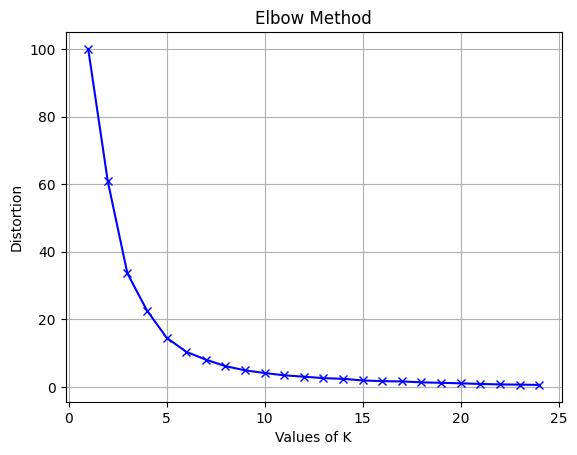
\includegraphics[width=0.45\linewidth]{elbow.png}
    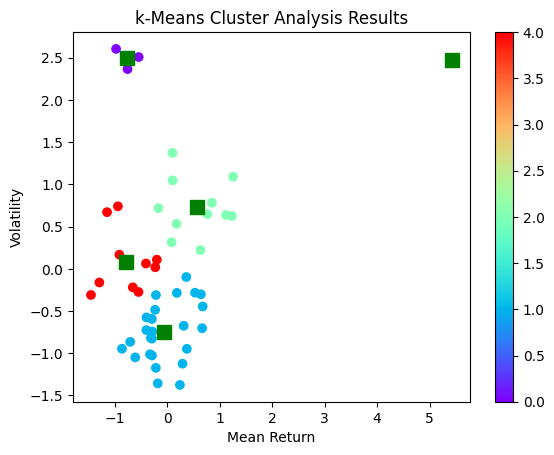
\includegraphics[width=0.45\linewidth]{clusters.png}
    \label{fig:enter-label}
\end{figure}

Then in each of the formed clusters, we looked at all stock pairs and ran a Cointegration Test on their stock values from 2018-22, that is if the p-value of a pair of stock was less than 0.5, we can say that they might be cointegrated. The number for these potential valid trading pairs came out to be 43. So now, to test if our potential valid trading pairs are actually profitable or not, we took each pair and their stock prices in 2023-24 and simulated the results as if they were a trading pair and calculated their Sharpe Ratio for this time. Sharpe Ratio, if comes out be positive, indicates positive returns for us and conversely if it is negative. Out of the 43 potential trading pairs, 23 pairs gave positive returns.

\begin{figure}[H]
    \centering
    \includegraphics[width=0.7\linewidth]{img1.png}
    \label{fig:enter-label}
\end{figure}

\section{References}
\begin{itemize}
    \item scikit-learn.org
    \item pytorch.org
    \item algotrading101.com
    \item kaggle.com
    \item machinelearningmastery.com
\end{itemize}
\end{document}